\chapter{Data preparation}

I want, at this point, to tell you something about the data that I got out of the detector, and how I fiddled with it to get the specific histogram, that I'm going to use to get my number out in the end.

Maybe at this stage, I should go back and remind myself what it is that I actually do...

\begin{figure}[htp]
\begin{minipage}[b]{.69\textwidth}
\hspace{-1em}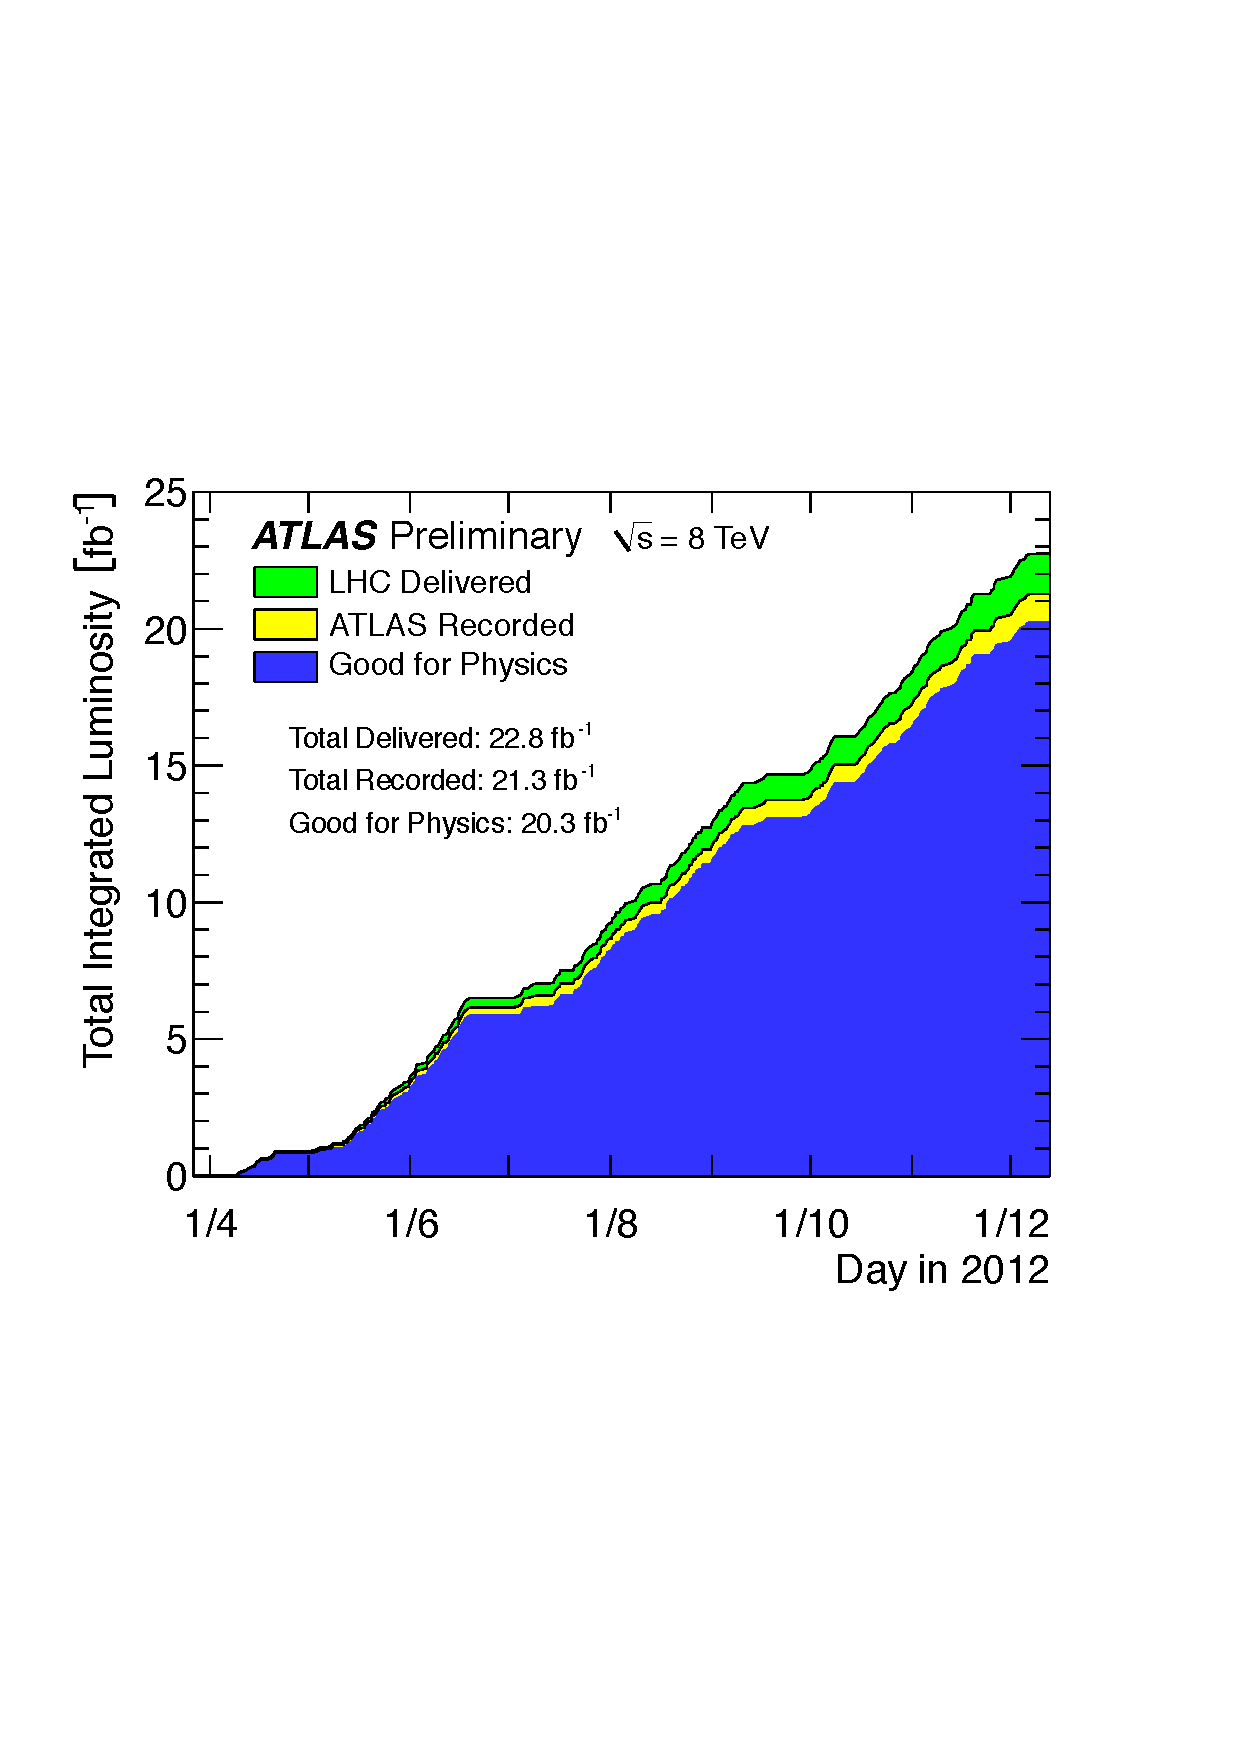
\includegraphics[width=\textwidth]{figures/intlumi}
\end{minipage}\hfill\begin{minipage}[b]{.3\textwidth}
\caption{A plot showing the integrated luminosity delivered by the LHC (green), recorded by ATLAS (yellow), and fulfilling data quality criteria (blue), over the course of the 8 TeV run in 2012 \cite{publiclumi}.
\label{intlumi}}
\end{minipage}
\end{figure}

I'll just throw some section headings at you, for now.

\section{Data from the detector}
We get \texttt{PHOTON_NTUP} root-files from \textsc{atlas}, where we've picked events that are loose, and have the proper $p_T$ and live in the correct $\eta$ ranges.

\section{Background filetering}
Then, knowing that background events have snuck their way into our data sample, we venture into some data-driven background subtraction methods. These will, if and when they work, be:

\subsection{The ABCD method}
Our old friend. And:

\subsection{The S-frame method}
Or however the hell you're supposed to render that. If it works.

Incidentally, the presence of pileup events probably means that we should run the MC events through this machinery as well. Even if we aren't filtering out the same things, we are filtering out \textit{some} of the same things, albeit, presumably, imperfectly(, natch). There are also things that aren't there, that we're not filtering out imperfectly, and so won't be there. But it's an imperfect world.

This should leave us with the sample of events that we will use to estimate $\Lambda$.
